% !TEX root = ../thesis_main.tex
%
%
%
\clearpage	
\chapter{Results and Conclusions}
\label{results_chapter}
%%%\note[jb1]{Me:
%%%\\
%%%My value of Abeta with bFierz=0 (which I see now that I haven't *actually* included in the text yet.  That clearly needs to happen.) is consistent with Ben's when you account for the fact that Ben's data is, on average, less polarized than he thought.  I think I mention this somewhere, but I probably need to make it more obvious, and located in the 'Conclusions' chapter.  
%%%\\ ... \\
%%%JB:
%%%\\
%%%thanks. Spot-on in your first paragraph--  you know what to do, you just need to write it down.
%%%}
\note[jb1]{JB:  Dan and I independently discussed (((Ch.~\ref{results_chapter}))) yesterday, and he has suggestions to
help. So I will also schedule a meeting with Dan and you to discuss
(((Ch.~\ref{results_chapter}))) Results and whether the S,T part must be deleted and left to a paper.
You don't have enough time, and although this should be quite straightforward,
it is not your critical result and it's the only thing that can go.}
\note[jb1]{JB on simple things still missing:
\\
%The final answers with uncertainties are only stated in the caption of Fig. 5.1.
I would have expected a separate uncertainty for b and Abeta for each data set,
either on each 2D figure in ch. 6, are collected in a table in Ch. 6.
}

\note{Remember to cite these dudes for (I think) the low-energy tail in the spectrum:  ~\cite{stragglingLonergan1970} \cite{stragglingRester1971}.}

%%% %%%%%%% %%%
%\section{Measured Limits on $b_{Fierz}$, $C_S$, $C_T$}
\section{Measured Limits on $b_{Fierz}$ and $\Abeta$}
\label{sec:measured_limits}
\note[jb1]{JB on Ch. ~\ref{sec:measured_limits}:
\\...\\
you just have to summarize the figures. Point out the natural dilution
of Abeta result if energy-dependent new physics is allowed to float.
}
%Results go here, with measured limits described and quantified in all formats anyone could ever care about.
\note[jb1]{John says to just skip doing the $C_S$ and $C_T$ stuff, for now.  No time.  ... Really, $C_S$ is already basically done, but then that'll lead to awkward questions about $C_T$.}

After corrections have been applied and uncertainties evaluated, statistical confidence intervals for the 2D $\Abeta$ vs $\bFierz$ parameter space are shown in Fig.~\ref{fig:2dchi2_alldata} for all datasets combined.  The final estimates of $\Abeta$ and $\bFierz$ with uncertainties at the $1\sigma$ level are given by:
\bea
\bFierz =& \,0.033  &\!\!\! \pm\, 0.084(\textrm{stat})\;\, \pm\, 0.039(\textrm{sys})  \\
\Abeta  =& -0.5738 &\!\!\! \pm\, 0.0082(\textrm{stat})    \pm\, 0.0041(\textrm{sys}), 
\eea
%
\begin{figure}[h!tb]
	\centering
	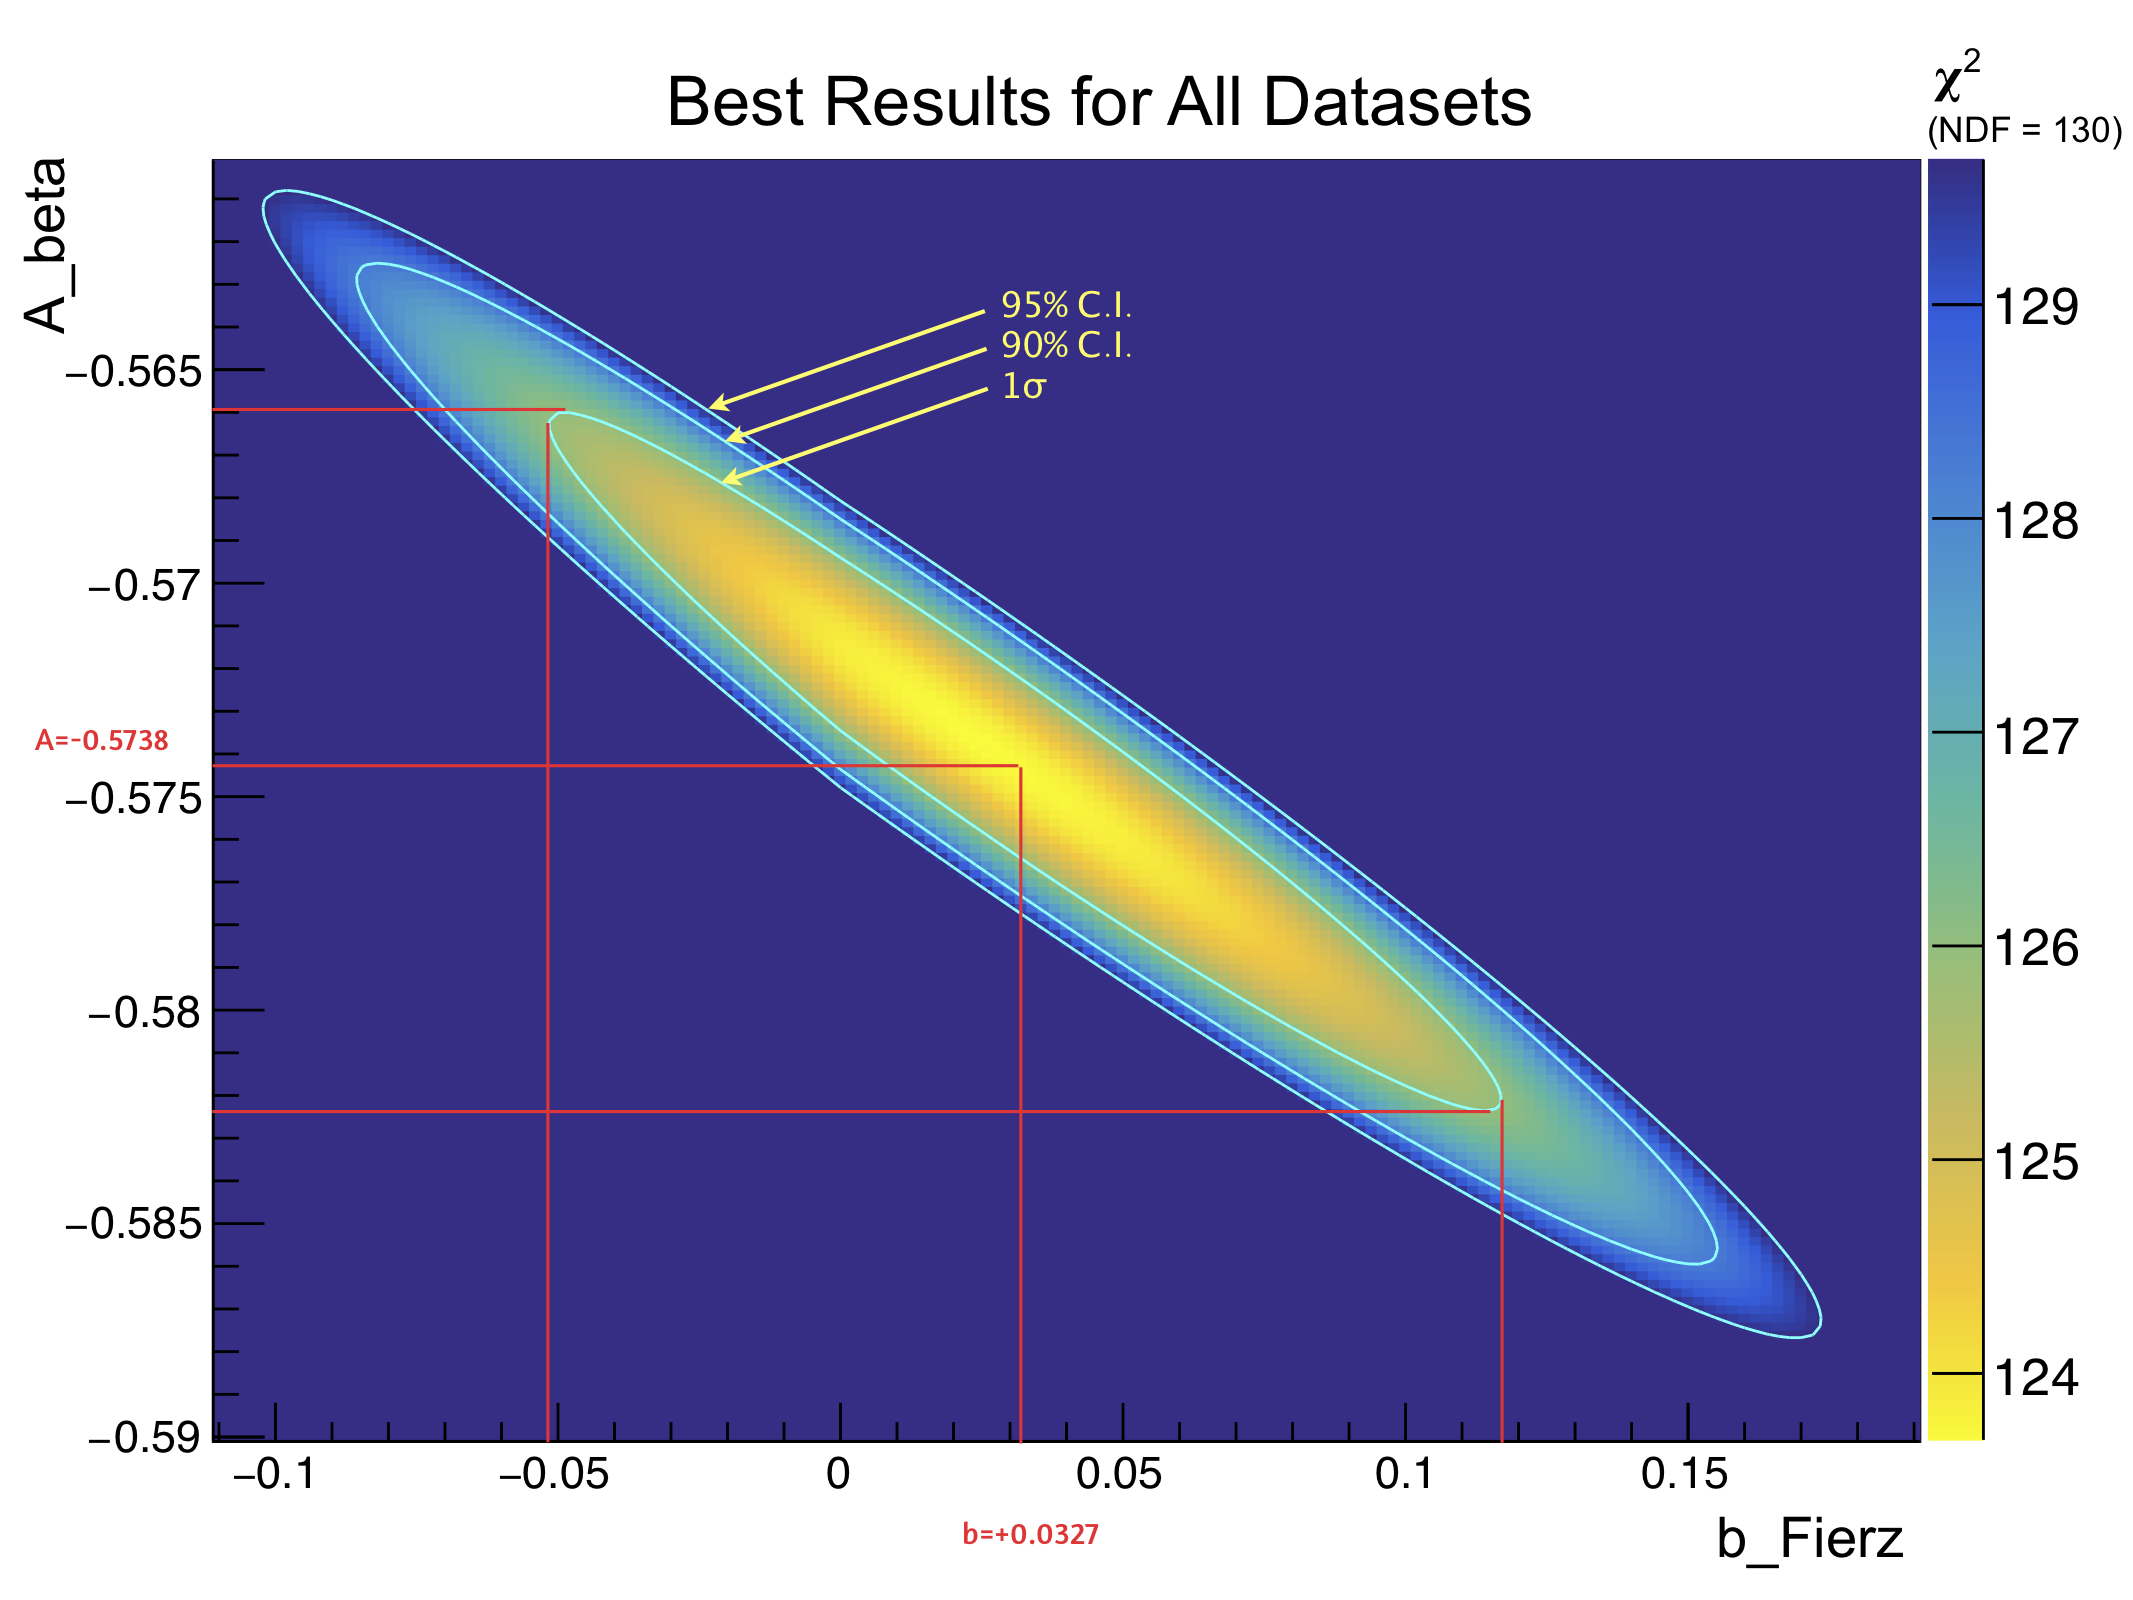
\includegraphics[width=.999\linewidth]
	{Figures/Chi2_2D_AllData.png}
	\caption[$\chi^2$ Map for All Data]{A $\chi^2$ map to compare all data to a parameter space of $\Abeta$ and $\bFierz$ values.  All corrections have been included, however only statistical confidence intervals are shown.}	
	\label{fig:2dchi2_alldata}
\end{figure}
%
and a list of uncertainties is provided in Table~\ref{table:budget}.
% !TEX root = ../thesis_main.tex



%%%% --- * --- %%%%	
%\renewcommand{\arraystretch}{1.6}

\begin{table}[h!!!!t]
	\begin{center}
	\begin{tabular}{ l  c  c  }
		\multicolumn{1}{l}{ Source} 		& \multicolumn{2}{c}{ \;\;\; \;\;\; Uncertainty \;\;\; \;\;\; }   
		\\
		\multicolumn{1}{l}{ } 				& \multicolumn{1}{c}{\;\; $\bFierz$}   & \multicolumn{1}{c}{$\Abeta$}   	
		\\  \hline
		%%% % %%%
		Scintillator Calibration 			& 0.003								& 0.0003											
		\\
		Scintillator Threshold  			& 0.004 							& 0.0004 						
		\\
		%%% % %%%
		DSSD Individual Strip SNR 			& 0.006								& 0.0007													
		\\
		DSSD Energy Agreement	  			& 0.005 							& 0.0006 						
		\\
		DSSD Detection Radius	  			& 0.006 							& 0.0017 						
		\\
		DSSD Energy Threshold	  			& 0.005 							& 0.0005 						
		\\
		%%% % %%%
		Atomic Cloud			  			& 0.002 							& 0.0002 						
		\\
		%%% % %%%
		Background				  			& 0.004 							& 0.0003 						
		\\
		%%% % %%%
		Beta Scattering				  		& 0.031 							& 0.0025 						
		\\
		%%% % %%%
		Low Energy Tail				  		& 0.008 							& 0.0007 						
		\\
		%%% % %%%
		Mirror Thickness				  	& 0.013 							& 0.0017 						
		\\
		DSSD Thickness				 	 	& 0.013 							& 0.0017 						
		\\
		Beryllium Foil Thickness			& 0.004								& $\!\!\!\!\!\! < 0.0001$ 			
	%	\\
		%%% % %%%
		\\  \hline
		\multicolumn{1}{l}{ Total Systematics} & \multicolumn{1}{c}{0.039}  & \multicolumn{1}{c}{0.0041}
%		Total Systematics			  		& 0.056 							& 0.0055 						
		\\
		\multicolumn{1}{l}{ Statistics} 	   & \multicolumn{1}{c}{0.084}  & \multicolumn{1}{c}{0.0082}
%		Statistics				  			& 0.084 							& 0.0082 						
	%	\\  \hline
		%%% % %%%
	\end{tabular}
	\end{center}
	\caption[Error Budget]{Error budget for the two-parameter analysis for $\bFierz$ and $\Abeta$, with all data included.  All uncertainties are believed to be uncorrelated, and are added in quadrature.  Final results: 
	$\mbox{ $\bFierz = 0.033 \pm 0.084(\textrm{stat}) \pm 0.039(\textrm{sys})$ }$ and $\mbox{ $\Abeta = -0.5738 \pm 0.0082(\textrm{stat}) \pm 0.0041(\textrm{sys})$ }$. }
	\label{table:budget}
\end{table}

%\renewcommand{\arraystretch}{1}



  %\label{table:budget}

The uncertainty associated with this measurement of $\Abeta$ is significantly larger than the collaboration's previous measurement of using the same data, in which the final result was $\mbox{$\Abeta = -0.5707 \pm 0.0013(\textrm{stat}) \pm 0.0013(\textrm{sys}) \pm 0.0005(\textrm{pol})$}$.  However, it must be noted that the present measurement is a two-parameter measurement rather than a one-parameter measurement, so it is expected to that the uncertainty associated with a single parameter should be larger.

To evaluate whether the two measurements are consistent, a thin vertical slice of Fig.~\ref{fig:2dchi2_alldata} can be extracted at $\bFierz=0$, and its projection will provide the centroid (including systematic offsets) and statistical error associated with a one-parameter analysis for $\Abeta$ -- though this method cannot produce an estimate of the extent to which systematic uncertainties might be reduced.  This `check' gives a one-parameter measurement of $\Abeta = -0.5714 \pm 0.0020(\textrm{stat})$.

The above one-parameter result for $\Abeta$ is consistent with the collaboration's prior result, even after one accounts for the fact that the previous result suffered from an oversight in which some partially polarized data was not removed from the final analysis for $\Abeta$, despite the fact that this cut \emph{was} implemented in the associated polarization measurement.  This accounts for $5\%$ of the data used in that analysis, and is estimated to decrease the average polarization by approximately $0.3\%$.  

An estimate of the size of the effect on the previous measurement of $\Abeta$ suggests that the true value of $\Abeta$ is likely to be $\sim 0.0016$ more negative than reported.  
%Furthermore, there is no uncertainty associated with polarization described within the present analysis, simply because to leading order there is no effect on $\bFierz$, although it strongly affects a measurement of $\Abeta$.  
Accounting for this, a more accurate one-parameter measurement might produce the result, $\mbox{$\Abeta \approx -0.5723 \pm 0.0014(\textrm{stat}) \pm 0.0013(\textrm{sys}) \pm 0.0005(\textrm{pol})$}$.


%%an oversight in data cut
%%when one accounts for the fact that an oversight in the previous analysis led to 
%Info on the $\Abeta$ measurement goes here too.  In particular, you set $\bFierz=0$ and see what happens to $\Abeta$.


%%% %%%%%%% %%%
%\section{Discussion of Corrections and Uncertainties}
\note{Kludgily removed an entire section:  ``Discussion of Corrections and Uncertainties''.  But comments from John on that section still remain.}
%\note[tag]{Write Discussion Section.}
\label{sec:discussion_corrections_uncertainties}
%\section{Overview}	
%A summary of systematics goes here.  In words, yes, but also in table form.
%%%\note[jb1]{JB on simple things still missing:
%%%\\
%%%I see no statement near Table ~\ref{table:budget} that you are adding the uncertainties in
%%%quadrature. As part of that you need a simple summary
%%%statement that all uncertainties are
%%%uncorrelated and, after the corrections applied, believed to be random. 
%%%}

%%%A list of uncertainties is provided in Table~\ref{table:budget}.
%%%% !TEX root = ../thesis_main.tex



%%%% --- * --- %%%%	
%\renewcommand{\arraystretch}{1.6}

\begin{table}[h!!!!t]
	\begin{center}
	\begin{tabular}{ l  c  c  }
		\multicolumn{1}{l}{ Source} 		& \multicolumn{2}{c}{ \;\;\; \;\;\; Uncertainty \;\;\; \;\;\; }   
		\\
		\multicolumn{1}{l}{ } 				& \multicolumn{1}{c}{\;\; $\bFierz$}   & \multicolumn{1}{c}{$\Abeta$}   	
		\\  \hline
		%%% % %%%
		Scintillator Calibration 			& 0.003								& 0.0003											
		\\
		Scintillator Threshold  			& 0.004 							& 0.0004 						
		\\
		%%% % %%%
		DSSD Individual Strip SNR 			& 0.006								& 0.0007													
		\\
		DSSD Energy Agreement	  			& 0.005 							& 0.0006 						
		\\
		DSSD Detection Radius	  			& 0.006 							& 0.0017 						
		\\
		DSSD Energy Threshold	  			& 0.005 							& 0.0005 						
		\\
		%%% % %%%
		Atomic Cloud			  			& 0.002 							& 0.0002 						
		\\
		%%% % %%%
		Background				  			& 0.004 							& 0.0003 						
		\\
		%%% % %%%
		Beta Scattering				  		& 0.031 							& 0.0025 						
		\\
		%%% % %%%
		Low Energy Tail				  		& 0.008 							& 0.0007 						
		\\
		%%% % %%%
		Mirror Thickness				  	& 0.013 							& 0.0017 						
		\\
		DSSD Thickness				 	 	& 0.013 							& 0.0017 						
		\\
		Beryllium Foil Thickness			& 0.004								& $\!\!\!\!\!\! < 0.0001$ 			
	%	\\
		%%% % %%%
		\\  \hline
		\multicolumn{1}{l}{ Total Systematics} & \multicolumn{1}{c}{0.039}  & \multicolumn{1}{c}{0.0041}
%		Total Systematics			  		& 0.056 							& 0.0055 						
		\\
		\multicolumn{1}{l}{ Statistics} 	   & \multicolumn{1}{c}{0.084}  & \multicolumn{1}{c}{0.0082}
%		Statistics				  			& 0.084 							& 0.0082 						
	%	\\  \hline
		%%% % %%%
	\end{tabular}
	\end{center}
	\caption[Error Budget]{Error budget for the two-parameter analysis for $\bFierz$ and $\Abeta$, with all data included.  All uncertainties are believed to be uncorrelated, and are added in quadrature.  Final results: 
	$\mbox{ $\bFierz = 0.033 \pm 0.084(\textrm{stat}) \pm 0.039(\textrm{sys})$ }$ and $\mbox{ $\Abeta = -0.5738 \pm 0.0082(\textrm{stat}) \pm 0.0041(\textrm{sys})$ }$. }
	\label{table:budget}
\end{table}

%\renewcommand{\arraystretch}{1}



  %\label{table:budget}

%	\section{Low-energy Scintillator Threshold}
%\aside{Choice of low-energy scintillator threshold has a large systematic effect...  
%\\...\\
%It's actually not nearly as big as I'd originally expected.  It's huge in the lineshape thing, but pretty tiny in everything else.}

%%%%\note[jb1]{from John:  ``I used Ben's threshold when determining the uncertainty from the lineshape tail (UFTLT). 
%%%%If you're saying the UFTLT depends on the threshold used, ok, of course it does. But if you're claiming that UFTLT depends on the **uncertainty** of the threshold, that's manifestly smaller than the UFTLT itself, and I'm going to assert it isn't worth evaluating.''}

%
\note{Just write a blurb to qualitatively summarize a bunch of the stuff in Ch.~\ref{systematics_chapter}.  Do I want to put my error budget table here?  If not, here it is! (~\ref{table:budget}). }
\note{Other things to discuss here:  which things are dominant error sources, and how viable it would be to improve those for future experiments.}


%%%\section{Relation to Other Measurements and New Overall Limits}
%%%\label{sec:relation_to_other_measurements}




%
%%%%%%% %%%%%%%%% %%%%%%%%
\clearpage
\section{Other Possible Future Work for the Collaboration:  $R_{\textrm{slow}}$}
\label{section_rslow}
\note{Probably shouldn't get a clearpage in the end.  It's for my sanity during writing.}
\note[jb1]{John says the whole $R_{\textrm{slow}}$ thing should go in here somewhere.}
\note[jb1]{Appendix I  keep, it's excellent. It should be moved as is to Conclusions under "Future Experiment for the collaboration"! so people know you worked so hard on it!!}
%\section{An Old Rslow Abstract}
The nuclear weak force is known to be a predominantly left-handed vector and axial-vector (V-A) interaction.  An experiment is proposed to further test that observation, constraining the strength of right-handed (V+A) currents by exploiting the principle of conservation of angular momentum within a spin-polarized beta decay process.  %\comment{
Here, we focus on the decay \mbox{$^{37}\textrm{K} \rightarrow \,^{37}\textrm{\!Ar} + \beta^{+} + \nu_e$}.  The angular correlations between the emerging daughter particles provide a rich source of information about the type of interaction that produced the decay.
%}

%, meaning that \comment{the fuck does it even mean?}, but limits are \comment{something something dark side}.  However, we are able to describe the probability distribution for the kinematics of the daughter particles in a beta decay reaction in terms of both right- and left-handed interactions, and scalar, tensor, vector, and axial couplings.  
%It is therefore possible to perform tests of the Standard Model by precisely measuring the kinematics within a beta decay process.  
%This document will focus predominantly on a search for right-handed interactions within the decay process, $^{37}\textrm{K} \rightarrow \,^{37}\textrm{\!Ar}^{+n} + \beta^{+} + \nu_e + (n+1)e^-$.

%{\color{cyan} (...) }

%\comment{ We obtain a sample of neutral, cold, nuclear spin-polarized $^{37}\textrm{K}$ atoms with a known spatial position, via the TRIUMF accelerator facility, by intermittently running a magneto-optical trap (MOT) to confine and cool the atoms, then cycling the trap off to polarize the atoms.  With $\beta$ detectors placed opposite each other along the axis of polarization, we are able to directly observe the momenta of $\beta^+$ particles emitted into 1.4\% of the total solid angle nearest this axis.  We also are able to extract a great deal of information about the momentum of the recoiling $^{37\!}$Ar daughters by measuring their times of flight and hit positions on a microchannel plate detector with a delay line.  Because the nuclear polarization is known to within $<0.1\%$~\cite{ben_OP}, and we are able to account for many systematic effects by periodically reversing the polarization and by collecting unpolarized decay data while the atoms are trapped within the MOT, we expect to be well equipped to implement a test of `handedness' within the nuclear weak force. }

%We have performed precision measurements of the kinematics of the daughter particles in the decay $^{37}\textrm{K} \rightarrow \,^{37}\textrm{\!Ar}^{+n} + \beta^{+} + \nu_e + (n+1)e^-$.
%\color{blue}
% of $^{37}$K.  This isotope decays by $\beta^+$ emission in a mixed Fermi/Gamow-Teller transition to its isobaric analog, $^{37\!}$Ar.  
%Because the higher-order standard model corrections to this decay process are well understood, it is an ideal candidate for for improving constraints on interactions beyond the standard model.  

%Our setup utilizes a magneto-optical trap to confine and cool samples of $^{37}$K, which are then released and spin-polarized by optical pumping.  
%This allows us to perform measurements on both polarized and unpolarized nuclei, which is valuable for a complete understanding of systematic effects.  
%Precision measurements of this decay are expected to be sensitive to the presence of right-handed vector currents, as well as a linear combination of scalar and tensor currents.  Progress towards a final result is presented here.
%\color{black}

\subsection{Motivation}
\label{rslow_motivation}

The nuclear weak force has long been known to be a predominantly left-handed chiral interaction, meaning that immediately following an interaction (such as a beta decay) with a weak force carrying boson ($W^+,\: W^-,\: Z$), 
%leptons emerge with left-handed chirality.  
normal-matter leptons (such as the electron and electron neutrino) emerge with left-handed chirality
% as seen from the decay frame, 
%\comment{(chirality?)}, chirality, 
while the anti-leptons (e.g. the positron and electron anti-neutrino) emerge with right-handed chirality.  
%\comment{(chirality?)}.  chirality.  
In the limit of massless particles, the particle's chirality is the same as its helicity. Thus, in a left-handed model, the direction of an (ultrarelativistic) normal lepton's spin is antiparallel direction of its motion, and the direction of spin for an anti-lepton is parallel to its direction of motion.  For a non-relativistic particle the property of chirality is fairly abstract, and describes the appropriate group representation and projection operators to be used in calculations.  It should be noted that a fully chiral model is also one which is maximally parity violating.
% \comment{(cite someone)}.

This odd quirk of the nuclear weak force is not only \emph{predominantly} true, but it is, to the best of our current scientific knowledge, \emph{always} true -- that is, attempts to measure any right-handed chiral components of the weak force have produced results consistent with zero~\cite{severijns_beck_cuncic_2006}\cite{severijns_cuncic_2011}.  This project proposes a further measurement to constrain the strength of the right-handed component of the weak interaction.  

%
%\section{The Principle of the Measurement}
%\label{principle}
%\comment{ Of particular interest is the decay process: $^{37}\textrm{K} \rightarrow \,^{37}\textrm{\!Ar} + \beta^{+} + \nu_e$.  Among other useful properties, this is is a `mirror' decay, 
%meaning that the nuclear wavefunctions of the parent and daughter are identical up to their isospin quantum number.  
%the number of protons in the parent nucleus (19) is equal to the number of neutrons in the daughter, and the number of neutrons in the parent (18) is equal to the number of protons in the daughter.  
%This property allows us to place strong constraints on the size of the theoretical uncertainties for this decay process within the Standard Model.   We further exploit this property by noting that both the $^{37}\textrm{K}$ parent and the $^{37}\textrm{\!Ar}$ daughter have nuclear spin $I=3/2$, a fact which is key to this experiment. }

%We propose to exploit the principle of conservation of angular momentum to search for right-handed currents.  Given a sample of cold, spatially confined, spin-polarized atoms which decay according to a known scheme, we propose to observe the kinematics of the daughter particles and thereby reconstruct beta decay event information.  
%
%In particular, given a fully spin-polarized ($m_I=\pm I$) 
%$\asdf37K$
%$^{37}\textrm{K}$ nucleus, the $^{37}\textrm{\!Ar}$ daughter may not take on a higher spin quantum number.  This puts a limit on the kinematics of the decay process.  If we assume, as per the Standard Model, that the spin-$1/2$ $\beta^+$ must emerge in a spin eigenstate parallel to its direction of motion (up to relativistic corrections), and that furthermore, the normal-matter $\nu_e$ must emerge with spin anti-parallel to its direction of motion.  Then, in the limiting case where the $\beta^+$ and the $\nu_e$ emerge exactly back-to-back, the Standard Model predicts that we will have changed the nuclear spin quantum number $m_I$ (as quantized along the `back-to-back' axis) by one unit.  However if, as per our assumption, the parent nucleus was already fully `spun up' in state $m_I = +3/2$, then $m_I$ may only decrease.
%
%In terms of beta decay kinematics, this means that given a $^{37}\textrm{K}$ nucleus which is spin-polarized to point upwards, if we observe a `back-to-back' decay along the axis of polarization, the Standard Model tells us that we can expect that the $\beta^+$ has gone upwards and the $\nu_e$ has gone downwards.  If we observe an event where the opposite is true, then we will have observed `new' physics beyond the predictions of the Standard Model (See Figure~\ref{fig:rhc}).  
%
%\begin{figure}[h!t]
%	\centering
%	\includegraphics[width=.999\linewidth]
%	{Figures/RHC_verbose2.png}
%	\caption{ A list of the `back-to-back' polarized $\beta^+$ decays in a simplified one-dimensional geometry.  The decays are labelled according to the type(s) of interaction that could produce them (vector, axial vector, scalar, and tensor).  By fully spin-polarizing the parent nucleus in a mirror decay, we are able to exclude diagrams (a) and (b).  Diagram (c), which represents the `left-handed' linear combination of vector and axial vector interactions, is the only one of these processes allowed within the Standard Model. Subfigure (d) represents the `right-handed' combination of vector and axial vector interactions.  Subfigures (e), (f), (g), and (h) could be produced by linear combinations of scalar and tensor interactions, neither of which have been observed within the Standard Model.  
%Within our experimental set-up we do not measure the spin of daughter particles directly, and therefore the decays in the top row (a, c, e, g) would be indistinguishable from one another, and decays in the bottom row (b, d, f, h) would also be indistinguishable from one another.  However since none of the latter event types would be possible under the Standard Model, an observation of this event type would be indicative of the presence of scalar, tensor, or right-handed interactions within the nuclear weak force. 
%\comment{(top and bottom rows are what's distinguishable in our experiment.)}
%}	
%	\label{fig:rhc}
%\end{figure}
%
%The problem, then, becomes one of designing an experiment which will allow us to isolate beta decay events with the desired signature from the more mundane beta decay events predicted by the Standard Model.  



%\pagebreak

%
%\section{The Experimental Setup}
%\label{setup}
%
%\color{usedcolor}
%\subsection{Overview}
%\label{overview}
%
%\begin{figure}[t!h]
%	\centering
%	\includegraphics[width=.999\linewidth]
%	{Figures/doublemot4.pdf}
%	\caption{The TRINAT experimental set-up utilizes a two MOT system in order to reduce background in the detection chamber.}	
%	\label{fig:doublemot}
%\end{figure}
%
%The TRIUMF Neutral Atom Trap (TRINAT) offers an experimental set-up which is uniquely suited to precision tests of Standard Model beta decay physics.  Radioactive ions are delivered from the ISAC beamline and neutralized before being trapped in the first of two magneto-optical traps (MOTs).  Approximately once per second, atoms from the first MOT are transferred to the second, where their decay products can be observed with significantly less background than would have been possible in the first trap (see Figure~\ref{fig:doublemot}).  The transfer methodology is discussed in some detail in a paper by Swanson et al~\cite{swanson}.
%
%Once the newly transferred atoms -- in this case, neutral $^{37}\textrm{K}$ -- have arrived at the second trap, the MOT cycles 500 times between a state where it is `on' and actively confining atoms to a region of approximately 2\,mm$^3$, to a state where it is `off' and instead the atoms are spin-polarized by optical pumping while the atom cloud expands ballistically before being re-trapped.  In order to eliminate systematic effects, the polarization direction is flipped every 16 seconds.  This optical pumping technique and its results are the subject of a recent publication~\cite{ben_OP}.
%
%The science chamber (shown in Figure \ref{fig:thechamber}) operates at ultra-high vacuum (UHV) and provides the apparatus necessary to intermittently confine atoms within a MOT and then spin-polarize them, and quantify their position, temperature, and initial polarization, and electrostatic hoops to allow for collection and observation of charged recoiling daughter nuclei, as well as further detectors to observe the outgoing betas and reconstruct angular correlations.  
%\comment{(should I elaborate here?) -- "no".} 
%
%\begin{figure}[h!!!tb]
%	\centering
%	\hspace*{\fill}%
%	\subfloat[A decay event within the TRINAT science chamber.  After a decay, the daughter will be unaffected by forces from the MOT.  Positively charged recoils and negatively charged shake-off electrons are pulled towards detectors in opposite directions.  Although the $\beta^+$ is charged, it is also highly relativistic and escapes the electric field with minimal perturbation.
%	%\comment{The pic is still kind-of fuzzy.}
%	]
%	{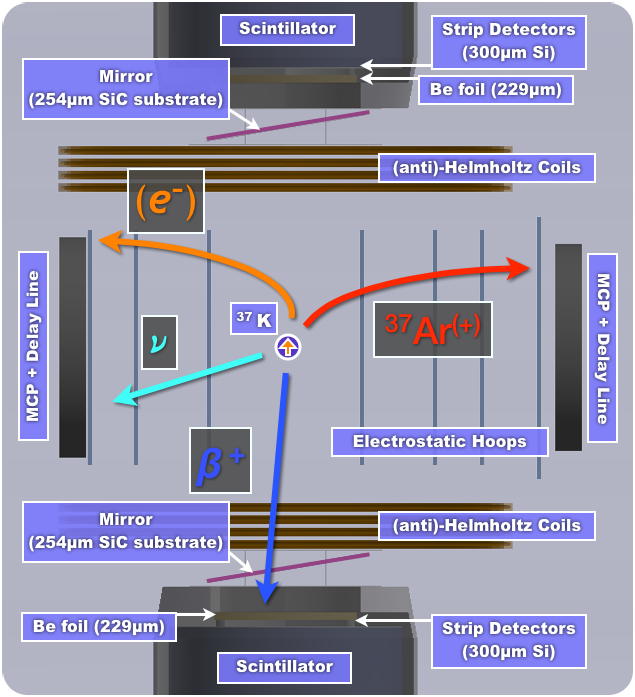
\includegraphics[width=.530\linewidth]{Figures/chamber_decayevent3.png}\label{chamber_decayevent} }
%	\hspace*{\fill}
%	\hfill
%	\hspace*{\fill}
%	\subfloat[Inside the TRINAT science chamber.  This photo is taken from the vantage point of one of the microchannel plates, looking into the chamber towards the second microchannel plate.  The current-carrying copper Helmholtz coils and two beta telescopes are visible at the top and bottom.  The metallic piece near the center is one of the electrostatic `hoops' used to generate an electric field within the chamber.  The hoop's central circular hole allows access to the microchannel plate, and the two elongated holes on the sides allow the MOT's trapping lasers to pass unimpeded at an angle of 45 degress `out of the page'.]	
%	{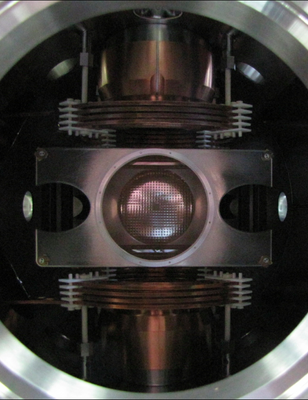
\includegraphics[width=.444\linewidth]{Figures/chamber_photo_2.png}}
%	\hspace*{\fill}%
%	\caption{The TRINAT detection chamber}	
%	\label{fig:thechamber}
%\end{figure}
%\clearpage
%\color{black}
%
%\subsection{Trapping}
%\label{trap}
%The Magneto-Optical Trap is a well-known technique from atomic physics, used to confine and cool neutral atoms~\cite{raabprentiss}.  The technique is used predominantly with alkalis due to their simple orbital electron structure, and is quite robust, so is appropriate for use with $^{37}\textrm{K}$.  Once set up, the trapping force is specific to the isotope for which the trap has been tuned, which makes it ideal for use in radioactive decay experiments, since the daughters are unaffected by the trapping forces keeping the parent confined.
%
%There are two primary components necessary for any MOT:  a laser, and a magnetic field.  The laser, which must be circularly polarized in the appropriate directions and tuned slightly to the red of an atomic resonance, is split into three perpendicular retroreflected beams, doppler cooling the atoms and (with the appropriate magnetic field) confining them in all three dimensions (see Figure~\ref{fig:mot}).  The TRINAT science chamber includes 6 `viewports' specifically designed to be used for the trapping laser.
%
%A MOT also requires a quadrupolar magnetic field, which we generate with two current-carrying anti-Helmholtz coils located within the vacuum chamber itself.  The coils themselves are hollow, and are cooled continuously by pumping temperature-controlled water through them.   
%
%One feature which makes our MOT unusual has been developed as a result of our need to rapidly cycle the MOT on and off -- that is, it is an ``AC-MOT''.  Rather than running the trap with one particular magnetic field and one set of laser polarizations to match, we run a sinusoidal AC current in the magnetic field coils, and so the sign and magnitude of the magnetic field alternate smoothly between two extrema, and the trapping laser polarizations are rapidly swapped to remain in sync with the field~\cite{harveymurray}\cite{thesis}.  See Figure~\ref{fig:acmot}.  
%
%\begin{figure}[ht]
%	\centering
%	\subfloat[Components of a magneto-optical trap, including current-carrying magnetic field coils and counterpropagating circularly polarized laser beams.]
%	{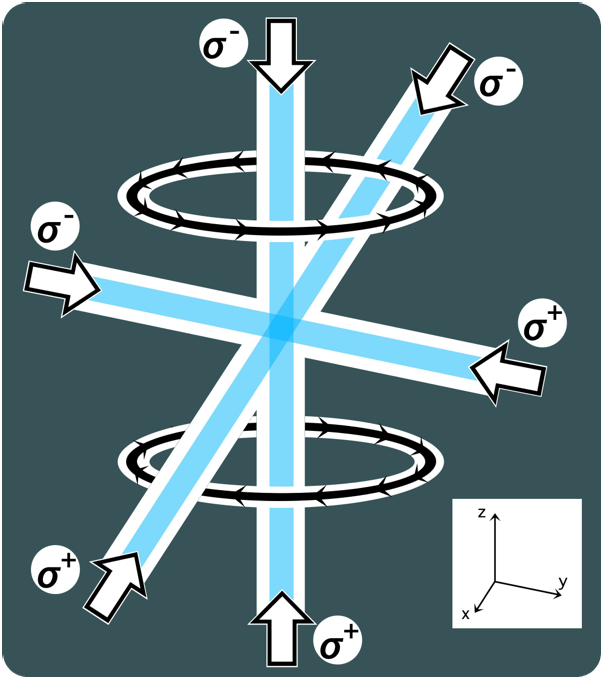
\includegraphics[width=.237\linewidth]{Figures/mot.png}\label{fig:mot} }
%	\hspace*{\fill}
%%	\hfill
%	\hspace*{\fill}
%	\subfloat[One cycle of trapping with the AC-MOT, followed by optical pumping to spin-polarize the atoms.  After atoms are transferred into the science chamber, this cycle is repeated 500 times before the next transfer.  The magnetic dipole field is created by running parallel (rather than anti-parallel as is needed for the MOT) currents through the two coils.]	
%	{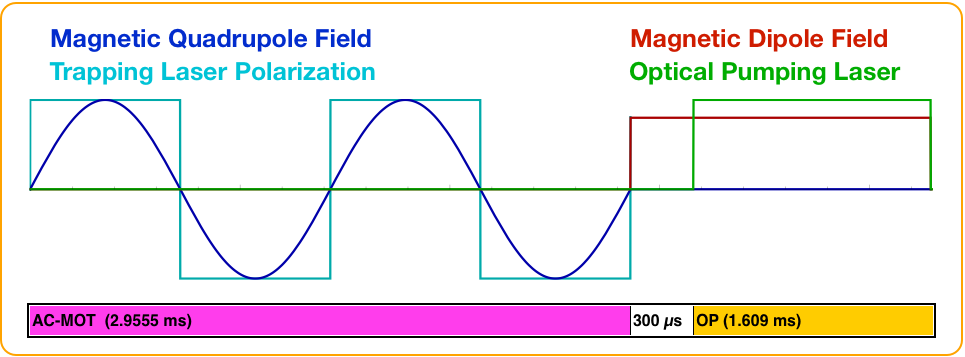
\includegraphics[width=.726\linewidth]{Figures/acmot.png}\label{fig:acmot} }
%	\caption{An alternating-current magneto-optical trap with a duty cycle optimized for producing polarized atoms}	
%	\label{fig:themot}
%\end{figure}
%
%The need to use an AC-MOT rather than a typical MOT has arisen as a direct result of our desire to optimally polarize our sample of atoms.  Polarization is incompatible with the non-uniform magnetic field used by a MOT, and rapidly shutting off the current used to produce the MOT's magnetic field produces eddy currents in the surrounding materials, which in turn produce their own non-uniform magnetic field in the region of interest.  The AC-MOT is developed as a way to ensure that the unavoidable eddy currents are behaving as we expect.  With an appropriate choice of shut-off phase, the current in the coils can be shut off when the overall magnetic field is already zero, so that no further eddy currents are induced.   

%{\color{cyan} (...) (something about why we need to run an AC-MOT.) }

%%%  Cut here?  %%%
%Note that because the atoms within a MOT can be treated as following a thermal distribution, some fraction of the fastest atoms continuously escape from the trap's potential well.  Even with the most carefully-tuned apparatus, the AC-MOT cannot quite match a similar standard MOT in terms of retaining atoms.  The TRINAT AC-MOT has a `trapping half-life' of around 6 seconds, and although that may not be particularly impressive by the standards of other MOTs, it is more than adequate for our purposes.  $^{37}\textrm{K}$ itself has a radioactive half-life of only 1.6 seconds \comment{(cite someone)}, so our dominant loss mechanism is radioactive decay rather than thermal escape. \comment{(Cut this whole paragraph?)}
%%%     %%%     %%%
%\clearpage

%


%\subsection{Optical Pumping}
%\label{op}
%We spin-polarize $^{37}\textrm{K}$ atoms within the trapping region by optical pumping~\cite{ben_OP}.  A circularly polarized laser is tuned to match the relevant atomic resonances, and is directed through the trapping region along the vertical axis in both directions.  When a photon is absorbed by an atom, the atom transitions to an excited state and its total angular momentum (electron spin + orbital + nuclear spin) along the vertical axis is incremented by one unit.  When the atom is de-excited a photon is emitted isotropically, 
%%\comment{(is it still isotropic when it's polarized?  I bet it's not.)}
%so it follows that if there are available states of higher and lower angular momentum, the \emph{average} change in the angular momentum projection is zero.  If the atom is not yet spin-polarized, it can absorb and re-emit another photon, following a biased random walk towards complete polarization.  
%
%In order to optimally polarize a sample of atoms by this method, it is necessary to have precise control over the magnetic field.  This is because absent other forces, a spin will undergo Larmor precession about the magnetic field lines.  In particular, the magnetic field must be aligned along the polarization axis (otherwise the tendency will be to actually depolarize the atoms), and it must be uniform in magnitude over the region of interest (otherwise its divergencelessness will result in the field also having a non-uniform direction, which results in a spatially-dependent depolarization mechanism).  Note that this type of magnetic field is not compatible with the MOT, which requires a quadrupolar magnetic field \emph{gradient}, and has necessitated our use of the AC-MOT as described in Subsection~\ref{trap}.


%\subsection{The Detectors}
%\label{detectors}
%\label{field}
%The beta detectors, located above and below the atom cloud along the axis of polarization (see Figure~\ref{chamber_decayevent}), are each the combination of a plastic scintillator and a set of silicon strip detectors.  Using all of the available information, these detectors are able to reconstruct the energy of an incident beta, as well as its hit position, and provide a timestamp for the hit's arrival.  Together the upper and lower beta detectors subtend approximately 1.4\% of the total solid angle as measured with respect to the cloud position. 
%
%It must be noted that the path between the cloud of trapped atoms and either beta detector is blocked by two objects:  a 254$\,\mu$m silicon carbide mirror (necessary for both trapping and optical pumping), and a 229$\,\mu$m beryllium foil (separating the UHV vacuum within the chamber from the outside world).  In order to minimize beta scattering and energy attenuation, these objects have had their materials selected to use the lightest nuclei with the desired material properties, and have been manufactured to be as thin as possible without compromising the experiment.  As the $^{37}\textrm{K} \rightarrow \,^{37}\textrm{\!Ar} + \beta^{+} + \nu_e$ decay proceess releases $Q=5.125$\,MeV of kinetic energy~\cite{Q_value}, the great majority of betas are energetic enough to punch through both obstacles without significant energy loss before being collected by the beta detectors.  
%
%On opposing sides of the chamber, and perpendicular to the axis of polarization, two stacks of $\sim$ 80\,mm diameter microchannel plates (MCPs) have been placed (see Figure~\ref{fig:thechamber}) as detectors, providing a time stamp when a particle is incident on their surfaces.  Behind each stack of MCPs there is a set of delay lines, which provide  position sensitivity for these detectors.   
%
%In order to make best use of these MCPs, we create an electric field in order to draw positively charged particles into one MCP, while drawing negatively charged electrons into the other MCP.  Seven electrostatic hoops have been placed within the chamber (see Figure~\ref{fig:thechamber}), and are connected to a series of high voltage power supplies.  See Sections~\ref{photoions} and~\ref{pos_recoils} for a discussion of what sort of charged particles we expect to observe in these detectors and how they are created.  
%  
%%\comment{(Say something about field uniformity?)}
%
%Scientific data has been collected at field strengths of 395 V/cm, 415 V/cm, and 535 V/cm.  It should be noted that these field strengths are too low to significantly perturb any but the least energetic of the (positively charged) betas from the decay process, and these low energy betas would already have been unable to reach the upper and lower beta detectors due to interactions with materials in the SiC mirror and Be foil vacuum seal.  
%


%\subsection{Cloud Measurements via Photoionization}
%\label{cloud}
%\label{photoions}
%In order to measure properties of the trapped $^{37}\textrm{K}$ cloud, a 10\,kHz pulsed laser at 355\,nm is directed towards the cloud.  These photons have sufficient energy to photoionize neutral $^{37}\textrm{K}$ from its excited atomic state, releasing 0.77\,eV of kinetic energy, but do not interact with ground state $^{37}\textrm{K}$ atoms.  The laser is of sufficiently low intensity that the great majority of excited state atoms are \emph{not} photoionized, so the technique is only very minimally destructive.  
%
%Because an electric field has been applied within this region (see Section~\ref{field}) the $^{37}\textrm{K}^+$ ions are immediately pulled into the detector on one side of the chamber, while the freed $e^-$ is pulled towards the detector on the opposite side of the chamber.  Because  $^{37}\textrm{K}^+$ is quite heavy relative to its initial energy, it can be treated as moving in a straight line directly to the detector, where its hit position on the microchannel plate is taken as a 2D projection of its position within the cloud.  Similarly, given a sufficient understanding of the electric field, the time difference between the laser pulse and the microchannel plate hit allows for a calculation of the ion's initial position along the third axis.  
%
%With this procedure, it is possible to produce a precise map of the cloud's position and size, both of which are necessary for the precision measurements of angular correlation parameters that are of interest to us here.  However, it also allows us to extract a third, slightly more subtle and significantly more important measurement:  the cloud's \emph{polarization}.
%
%The key to the polarization measurement is that only atoms in the excited atomic state can be photoionized.  While the MOT runs, atoms are constantly being pushed around and excited by the trapping lasers, so this period of time provides a lot of information for characterizing the trap size and position.  When the MOT is shut off, the atoms quickly return to their ground states and are no longer photoionized until the optical pumping beam is turned on.  As described in Section~\ref{op}, and in greater detail in~\cite{ben_OP}, the optical pumping process involves repeatedly exciting atoms from their ground states until the atoms finally cannot absorb any further angular momentum and remain in their fully-polarized (ground) state until they are perturbed.  Therefore, there is a sharp spike in excited-state atoms (and therefore photoions) when the optical pumping begins, and none once the cloud has been completely polarized.  The number of photoion events that occur once the sample has been maximally polarized, in comparison with the size and shape of the initial spike of photoions, provides a very precise characterization of the cloud's final polarization~\cite{ben_OP}.



%\comment{Photoions, the MCP, polarization stats, camera.}
%{\color{cyan} (...) }

%
\subsection{The Decay Process}
\label{rslow_decayprocess}
\label{pos_recoils}
% % %
The kinematics of nuclear $\beta^+$ decay are described by the following probability density function:
\bea
\label{jtw_pdf}
W(\langle I \rangle | E_\beta \hat{\Omega}_\beta \hat{\Omega}_\nu) 
&=& \left(\frac{1}{2\pi}\right)^{\!5} \!\! F\!\left( - Z, E_\beta \right)\, 
p_\beta E_\beta (E_0 - E_\beta)^2 \textrm{d}E_\beta \textrm{d}\hat{\Omega}_\beta \textrm{d}\hat{\Omega}_\nu \, \xi 
%
\!\!\!\! \nonumber \\ && \times
\left[ 1 + a_{\beta\nu} \frac{\vec{p}_\beta \cdot \vec{p}_\nu}{E_\beta E_\nu}
+ b_{\textrm{Fierz}} \frac{m_e}{E_\beta} 
\phantom{\frac{\left(\vec{p}_\beta\right)^2}{\vec{p}_\beta}} 
%
\!\!\!\! \right. \nonumber \\ &&\left. 
+ \, c_\textrm{align} \left( \frac{\frac{1}{3}\vec{p}_\beta \cdot \vec{p}_\nu - (\vec{p}_\beta \cdot \hat{j}) ( \vec{p}_\nu\cdot \hat{j} ) }{E_\beta E_\nu} \right) \!
 \left( \frac{I(I+1) - 3\langle (\vec{I}\cdot\hat{i})^2 \rangle}{I(2I-1)} \right) 
%
\right. \nonumber \\ && \left. 
+ \frac{\langle \vec{I} \rangle}{I} \left( A_\beta\frac{\vec{p}_\beta}{E_\beta} + B_\nu \frac{\vec{p}_\nu}{E_\nu} + D_{\textrm{TR}} \frac{\vec{p}_\beta \times \vec{p}_\nu}{E_\beta E_\nu} \right)
\right],
\eea
where $\vec{I}$ is the nuclear spin-polarization, $F\!\left( - Z, E_\beta \right)$ is the Fermi function, 
and parameters $\xi$, $a_{\beta\nu}$, $ b_{\textrm{Fierz}}$, $c_\textrm{align}$, $A_\beta$, $B_\nu$, and $D_{\textrm{TR}}$ are functions that vary with the strengths of the vector, axial, scalar, and tensor couplings (constant throughout nature), as well as the Fermi and Gamow-Teller nuclear matrix elements (specific to the individual decay)~\cite{jtw}\cite{jtw_coulomb}.

%{\color{cyan} (...) }

The decay may be treated as a three-body problem in which the available kinetic energy is divided up between the beta, the neutrino, and the recoiling $^{37}\textrm{\!Ar}$ nucleus, and (of course) the total linear and angular momentum are conserved.  While the neutrino cannot be detected directly, its kinematics may be reconstructed from observations of the beta and the recoiling daughter nucleus.  By placing detectors above and below the decaying atom along the axis of its polarization, we are able to obtain information about the outgoing beta's energy and momentum, in the cases of interest to us, where it is emitted along (or close to) the axis of polarization.  

The recoiling $^{37}\textrm{\!Ar}$ nucleus is a bit trickier to work with, but the task is not impossible.  One useful feature of the $^{37}\textrm{K} \rightarrow \,^{37}\textrm{\!Ar}$ transition is that, in addition to the $\beta^+$ emitted in the decay itself, one or more \emph{orbital} electrons from the parent atom are typically lost.  In the majority of decay events
%\comment{(80\% of them?  Give a number.  Cite someone.  Dan's thesis?~\cite{dan_thesis}  Or Alexandre's talk from like 1999.)}, 
only one orbital electron is `shaken off' and so the daughter $^{37}\textrm{\!Ar}$ atom is electrically neutral~\cite{gorelov2000}\cite{dan_thesis}.  In the remaining cases, two or more orbital electrons are lost this way, and the daughter atom is positively charged.  If we apply an electric field perpendicular to the direction of polarization, these positively charged $^{37}\textrm{\!Ar}^{(+n)}$ ions may be collected into a detector, from which hit position and time of flight information may be extracted.  These shake-off electrons are emitted with an average energy of only $\sim$ 2\,eV
%very little kinetic energy ($\sim$ 2\,eV)
%\comment{(give a number.  2 eV?  I should check.  Also, do I cite one of John's talks here?)}, 
so to a very good approximation the other decay products are not perturbed by the presence of shake-off electrons.  

It should be noted that for the class of decays of greatest interest, where the beta and the neutrino emerge back-to-back along the polarization axis, the recoiling daughter nucleus will have zero momentum along the directions perpendicular to this axis, and on average less total energy than if the beta and neutrino were emitted in a parallel direction.  Henceforth, daughter nuclei from a back-to-back decay as shown in Figure~\ref{fig:rhc} will be described as `slow' recoils.  In terms of observables, this means that if the electric field is configured to point along one of the axes perpendicular to the polarization direction, then when the recoiling ion is swept away into a detector, the slow recoil's hit position should be exactly along the projection of the polarization axis.  Furthermore, the slow recoil's time of flight should be in the middle of the time of flight spectrum, since other recoils will be emitted with momentum towards or away from the detector.  
\note[gs]{ 10. P. 93 contains a reference to “Figure ??”  (that's actually the thing above, Figure~\ref{fig:rhc}, no matter what page it's on now.) }


%Of course, in any real experiment, the number of decays emitted in exactly one set of directions will be a set of measure zero.  \comment{(say something about the limits taken as beta decay events approach the optimal set of angles.  Or just delete this paragraph because it's stupid.)}
% % %

%\section{Proposed Project}
%\label{project}
%Using $^{37}\textrm{K}$ beta decay data collected in June 2014, I intend to reconstruct the recoil momenta both along the polarization axis and perpendicular to it, such that when combined with energy and hit position from the beta detectors, each event's full kinematics may be reconstructed.  The spectra created by these events will be compared against a series of Geant4-based Monte Carlo simulations.  
%
%Matched template fitting will be used to compare the experimental data to the simulation, meaning that the implicit vector, axial, scalar, and tensor couplings within Eq.~\ref{jtw_pdf} will be allowed to float separately within the simulation, and a series of simulation ``templates'' will be produced, and each separately fit to the data.  The quality of each fit will be used to determine a ``best'' experimental value for both parameters, as well as the error inherent in the measurement.  
%
%%{\color{cyan} (...) }
%%\comment{See Figure~\ref{fig:Rslow_tof} ?}
%\begin{figure}[h!!t]
%	\centering
%	\includegraphics[width=.999\linewidth]
%	{Figures/Rslow_tof_squished.png}
%	\caption{Time-of-flight spectra for charged $^{37}\textrm{\!Ar}$ recoils at 535 V/cm, sorted by whether the $\beta$ was detected after emerging \emph{with} or \emph{against} the nuclear polarization direction, compared against a simulation using a uniform electric field.  	Recoils with zero initial momentum along the flight axis arrive in the center of the distribution for their charge state.  
%	}	
%	\label{fig:Rslow_tof}
%\end{figure}

%
\subsection{Status of the $R_{\textrm{slow}}$ Measurement}
\label{rslow_status}
In June 2014, after several years of preparatory work beforehand (the author has been continuously involved with this project since 2010), approximately 7 days of beam time at TRIUMF was dedicated to the TRINAT $^{37}\textrm{K}$ beta decay experiment.  Approximately half of this data is suitable for use in this project.  During this period, approximately 10,000 atoms were held within the trap at any given time.  The cleaned spectra show around 50,000 polarized beta-recoil coincidence events in total, divided among measurements at three different electric field strengths (535 V/cm, 415 V/cm, 395 V/cm). 

%At the present time, analysis is underway.  The recoil MCP hit position data has been calibrated, and systematic effects in the trap position and size measurements are being considered.  The largest two remaining hurdles for the analysis both lie in improvements to the Monte Carlo.  

%The first challenge is to implement particle tracking within a \emph{non-uniform} electric field.  Using the true non-uniform electric field will shift the time-of-flight spectra overall by around 1\%, and is expected to change the \emph{shape} of spectra as well, since the deviation from uniformity changes significantly as a function of flight tragectory, and is greater the farther a particle ventures from the central axis.  This would affect the measured hit positions as well.  Taken together, the shape of the time-of-flight spectra (as in Figure~\ref{fig:Rslow_tof}) and the recoil hit position are critical to our reconstruction of the decay process, it is critical that we model them correctly.  

%The second challenge will be to allow our simulation to vary vector, axial, scalar, and tensor coupling constants separately while holding other physical parameters (such as the half-life and Fermi/Gamow-Teller ratio) constant.  This, too, will be absolutely critical to the analysis, and its implementation is likely to be non-trivial.

A fit to simulation has shown that the data that has already been collected has sufficient statistical power to measure the \emph{fractional} contribution of any polarized `new physics' beta decay parameter (ie right-handed, scalar, and tensor currents within the weak interaction) to a sensitivity of $\sim 2\%$ of its true value.  Systematic limitations are still being assessed.  
%Because previous measurements have already shown that any $(V-A)$, $S$, and $T$ terms within the Standard Model must be quite small~\cite{severijns_beck_cuncic_2006}\cite{severijns_cuncic_2011}, the present measurement is not likely to be able to add any new constraints to our understanding of Standard Model physics, and must instead be understood as complementary to previous measurements.
%Because previous measurements have 
%Quantifying this observable's sensitivity to physics beyond the Standard Model in comparison to previously measured constraints~\cite{severijns_beck_cuncic_2006}\cite{severijns_cuncic_2011} is work in progress.  



%Approximately of beamtime and several years of preparatory work beforehand, and its analysis is currently underway.  The statistical strength of our data is sufficient for a \comment{5\%?  (John said 5\%, but I don't really know how he calculated that...)} measurement to constrain right-handed weak interactions, however the systematic effects within the data have not yet been fully evaluated.  This constraint is far too weak to allo w for the discovery of a right-handed component of the nuclear weak force, and is likely also too weak to place any new constraints on its strength.  It could, at best, lend statistical strength to the constraints on right-handed currents that have already been observed.
%
%Unfortunately, due to beam scheduling and target creation procedures at TRIUMF, and because several components of the TRINAT science chamber have subsequently been removed and disassembled to prepare for future upgrades to the apparatus, it would be extremely difficult to collect any further data in a timely fashion.  

%\pagebreak





%%%%%% %%%%%%% %%%%%%%
\section{Conclusions}
This two-parameter analysis to measure $\Abeta$ and $\bFierz$ has produced the results:
\bea
\bFierz =& \,0.033  &\!\!\! \pm\, 0.084(\textrm{stat})\;\, \pm\, 0.039(\textrm{sys})  \\
\Abeta  =& -0.5738 &\!\!\! \pm\, 0.0082(\textrm{stat})    \pm\, 0.0041(\textrm{sys}),
\eea
where uncertainties are evaluated at 1$\sigma$.  This measurement of $\bFierz$ is consistent with the Standard Model value of $\bFierz=0$, and $\Abeta$ is consistent both with the collaboration's prior measurement of $\Abeta$, as well as with the value predicted by the Standard Model at $\Abeta=-0.5706\pm0.0007$.

The result for $\bFierz$ is dominated by statistical uncertainty, suggesting that the measurement could be improved simply by counting longer.  There is also room for improvement in the systematic uncertainty, which is dominated by scattering and the related measurements of material thicknesses.  

\note[jb1]{JB on Ch. \ref{sec:discussion_corrections_uncertainties} -- `discussion of corrections and uncertainties':
\\...\\
could be as simple as
"The bFierz result in Table 5.1 is dominated by statistical uncertainty.
Largely because of this result,
the collaboration is working to reduce the largest systematics,
using lower-Z materials to reduce backscattering, and changing the silicon
delta-E to a multi-wire proportional chamber with very thin windows.
The collaboration has already implemented very thin pellicle mirrors.
The projected systematic uncertainty could approach 0.01 in a future
experment, which would then likely continue to be limited by statistics."
\\...\\
or all of that could go at the end of Chapter 5.
}
\note[tag]{put in that thing John said.}

%%%%%\note[jb1]{JB on simple things still missing:  
%%%%%\\
%%%%%In Conclusions:
%%%%%\\...\\
%%%%%Comparing bFierz to theory value of 0,  bFierz is (in)consistent with SM
%%%%%at Z sigma.
%%%%%\\...\\
%%%%%Comparing Abeta  and Abeta(theory) the result is (in)consistent with SM at X\% and Y sigma.
%%%%%}
%%%%%
%%%%%%%%Conclusions go here.
%%%%%
































